\documentclass{article}
\usepackage{ctex}
\usepackage{graphicx}

\title{MODIS数据下载简要说明}
\author{董昱}
\date{\today}

\graphicspath{{pictures/}}


\begin{document}
	\maketitle
	以下以MODIS的NPP为例,简要说明下载流程。
	\section{App Key的生成}
	首先登陆https://ladsweb.nascom.nasa.gov/search/,需要注册一个账号,在网页的右上角单击Profile按钮,选择AppKeys。
	
	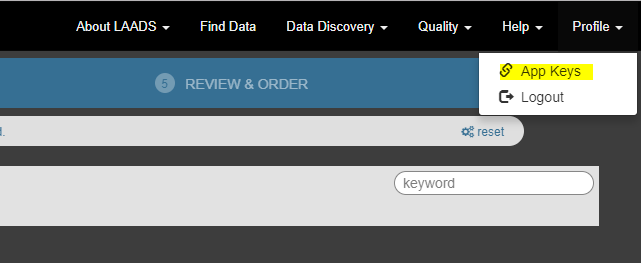
\includegraphics[width=6cm]{sec1_1.PNG}
	
	在弹出的页面中,随意输入Description,单击"Create New App Key"按钮,生成一个App Key,请在下方的表格中记下这个App Key,后面会用到。
	
	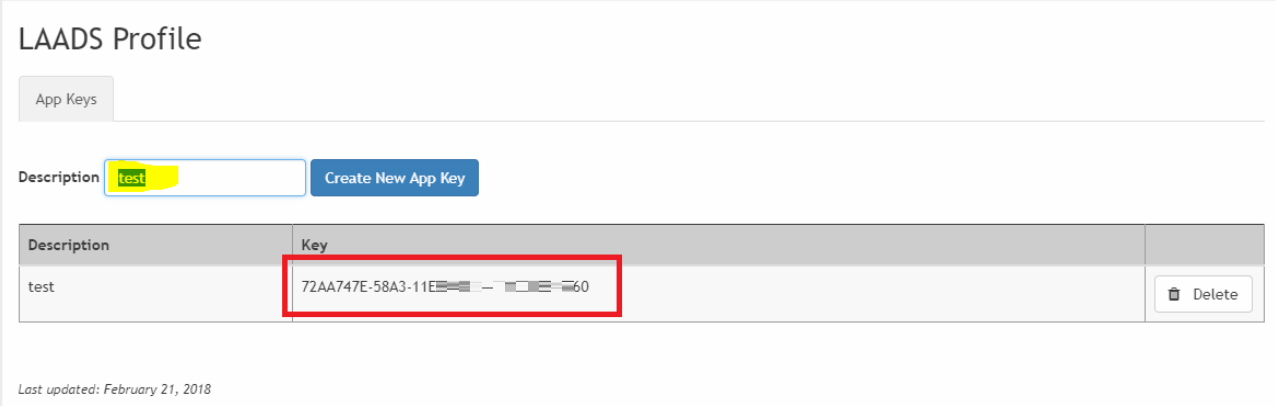
\includegraphics[width=\linewidth]{sec1_2.png}
	
	\section{数据资源选择}
	
	\subsection{产品选择}
	
	卫星选择MODIS:Terra, Collection选择6 - MODIS Collection 6。如果要下载NDVI数据,选择Vegetation Indices下面的MOD13A1/Q1/A2/A3。如果要下载NPP数据,可选择"GPP \& NPP" 下面的MOD17A2H。
	
	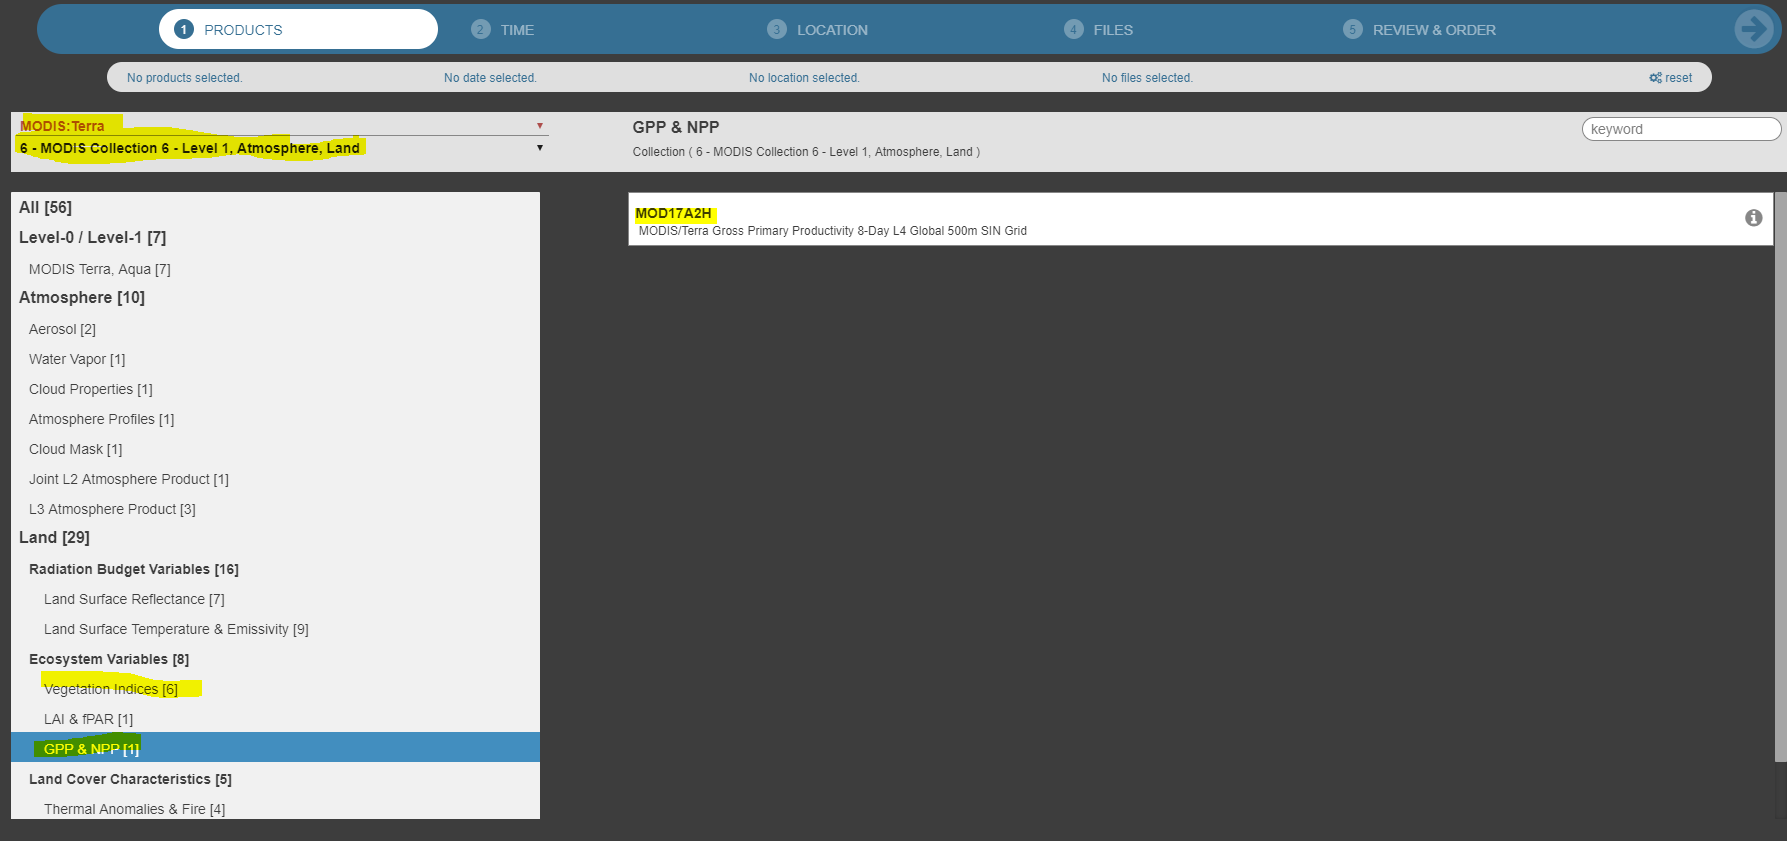
\includegraphics[width=\linewidth]{sec2_1.png}
	
	\subsection{时间选择}
	
	略
	
	\subsection{位置选择}
	
	可以利用Tiles等方法选择下载数据的区域。
	
	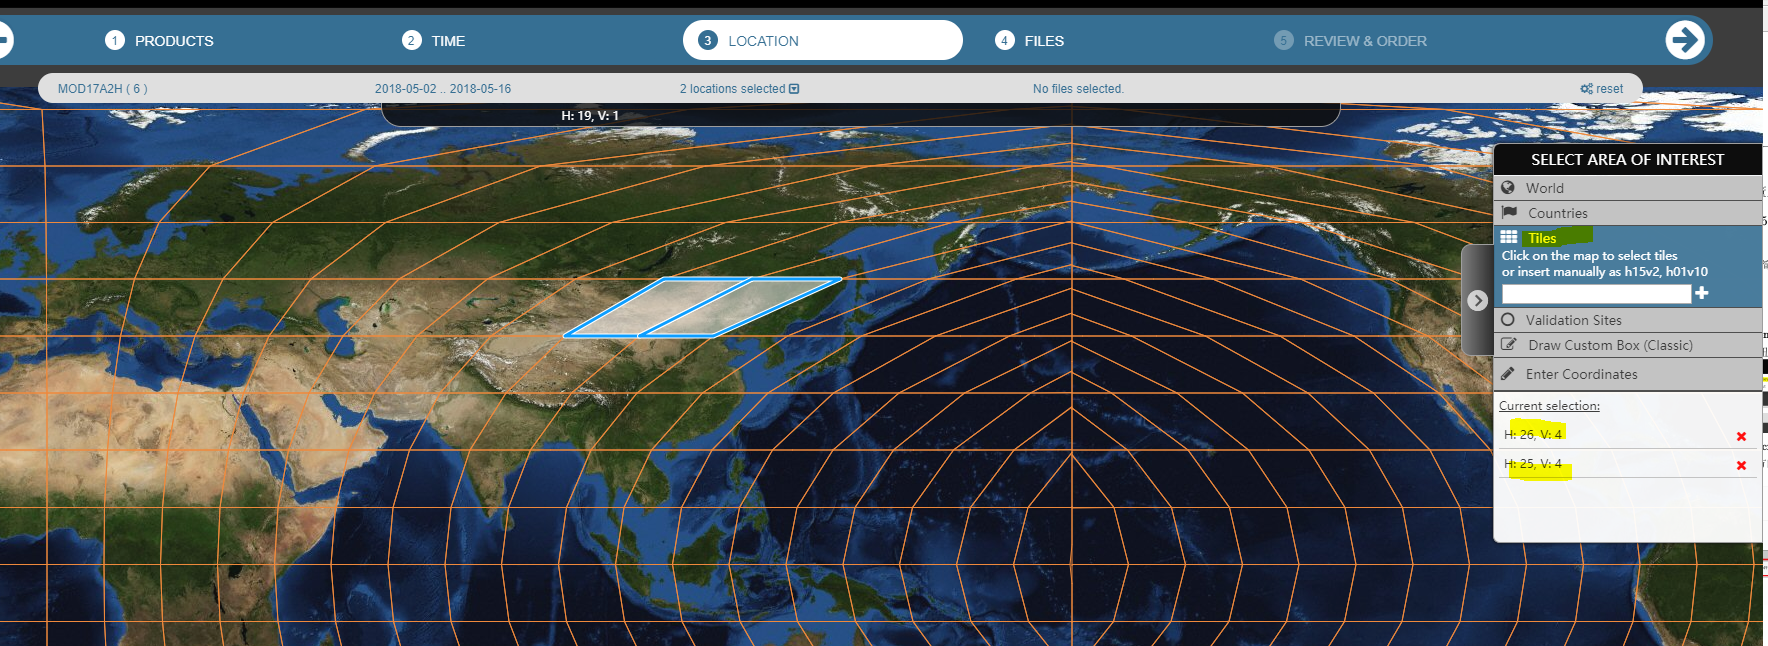
\includegraphics[width=\linewidth]{sec2_2.png}
	
	\subsection{数据文件选择}
	
	在这个页面中,检查时间与位置的选择是否正确,文件的数量是否正确。如果正确,单击“Select All”选择全部数据。
	
	在右侧Download列下,可以下载单个的数据。
	
	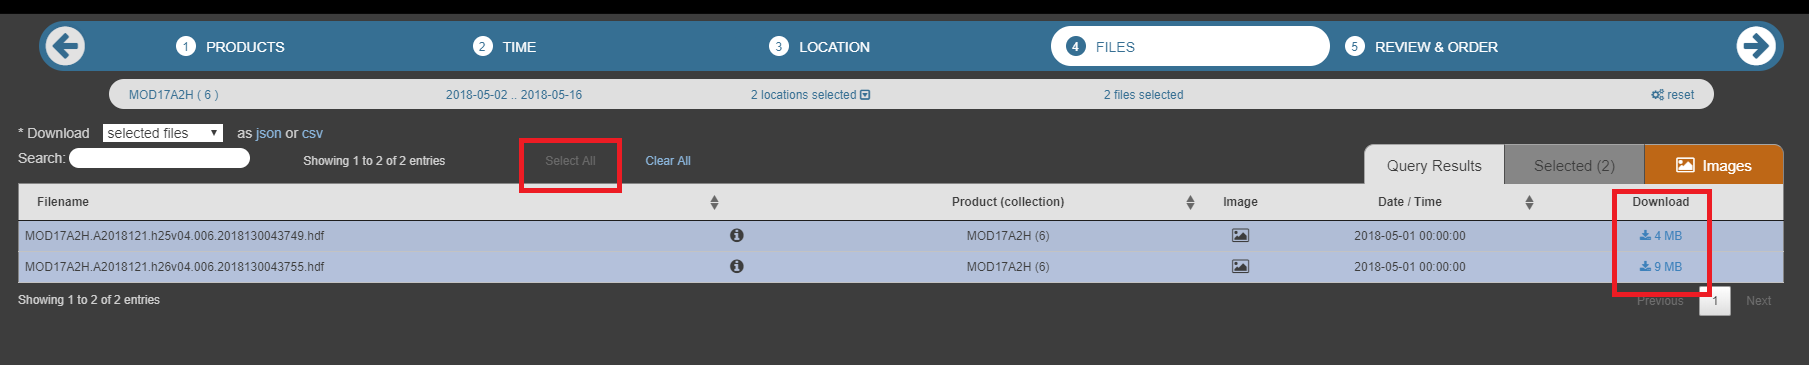
\includegraphics[width=\linewidth]{sec2_3.png}
	
	\subsection{数据提交}
	
	在这个页面中,在"Select Delivery Method"下面选择"Pull",然后单击"Submit Order"按钮提交。
	
	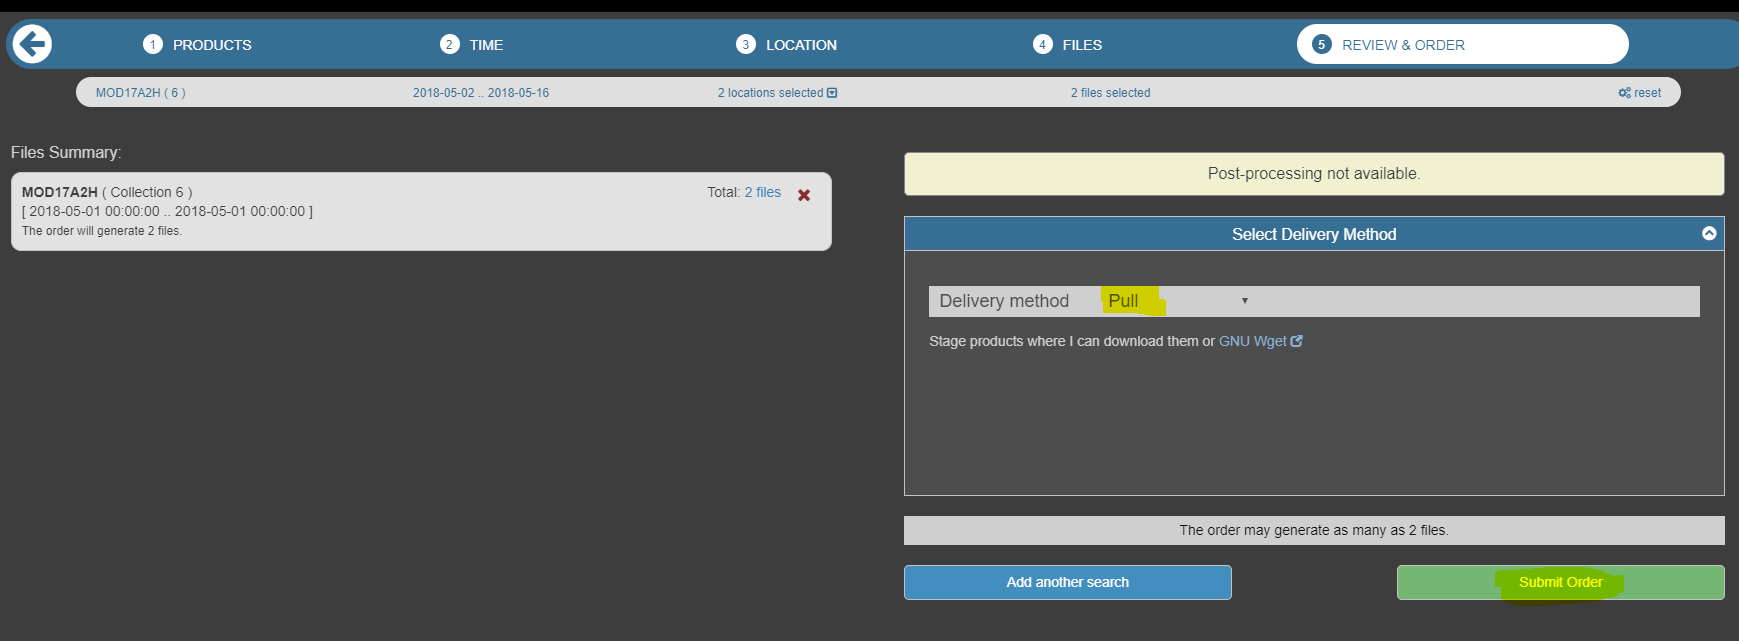
\includegraphics[width=\linewidth]{sec2_4.png}

	\section{Wget的配置}
	
	\subsection{Wget的下载}
	在https://eternallybored.org/misc/wget/页面中下载Wget的最新版本。
	
	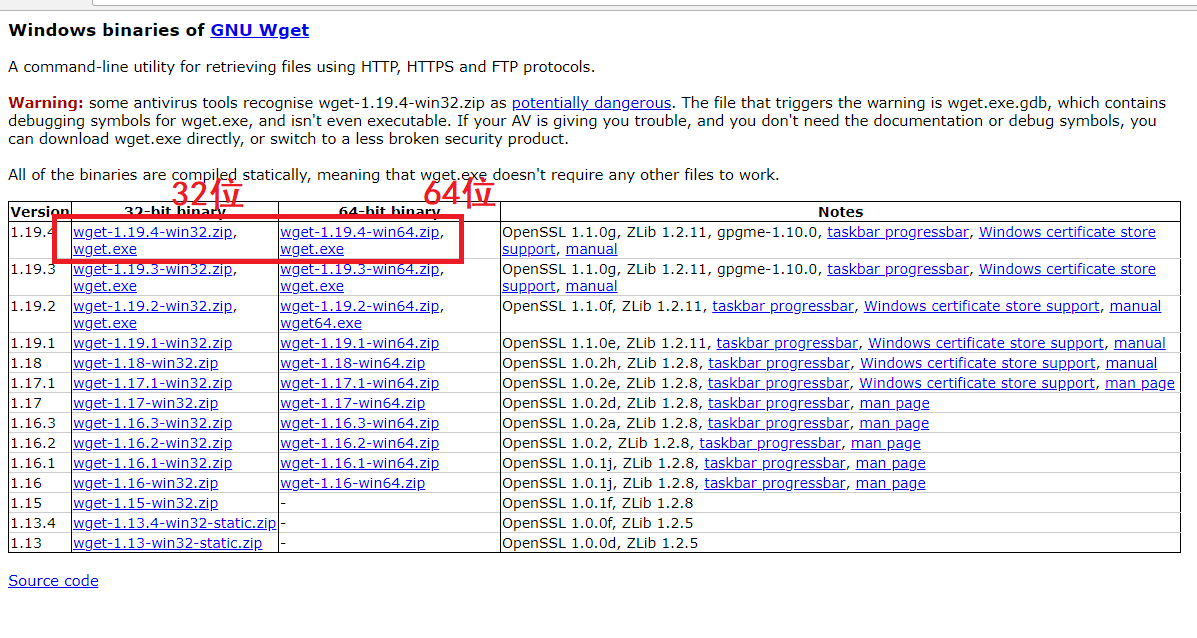
\includegraphics[width=\linewidth]{sec3_1.png}
	
	解压文件,找到wget.exe文件。
	
	\subsection{Wget环境变量配置}
	
	在计算机(或者"我的电脑")上单击鼠标右键,选择属性按钮。在弹出的对话框中单击"高级系统设置",选择"高级"选项卡,单击下方的"环境变量"按钮,找到系统变量下面的Path变量,双击进行编辑,添加wget.exe文件所在的目录,之后保存。
	
	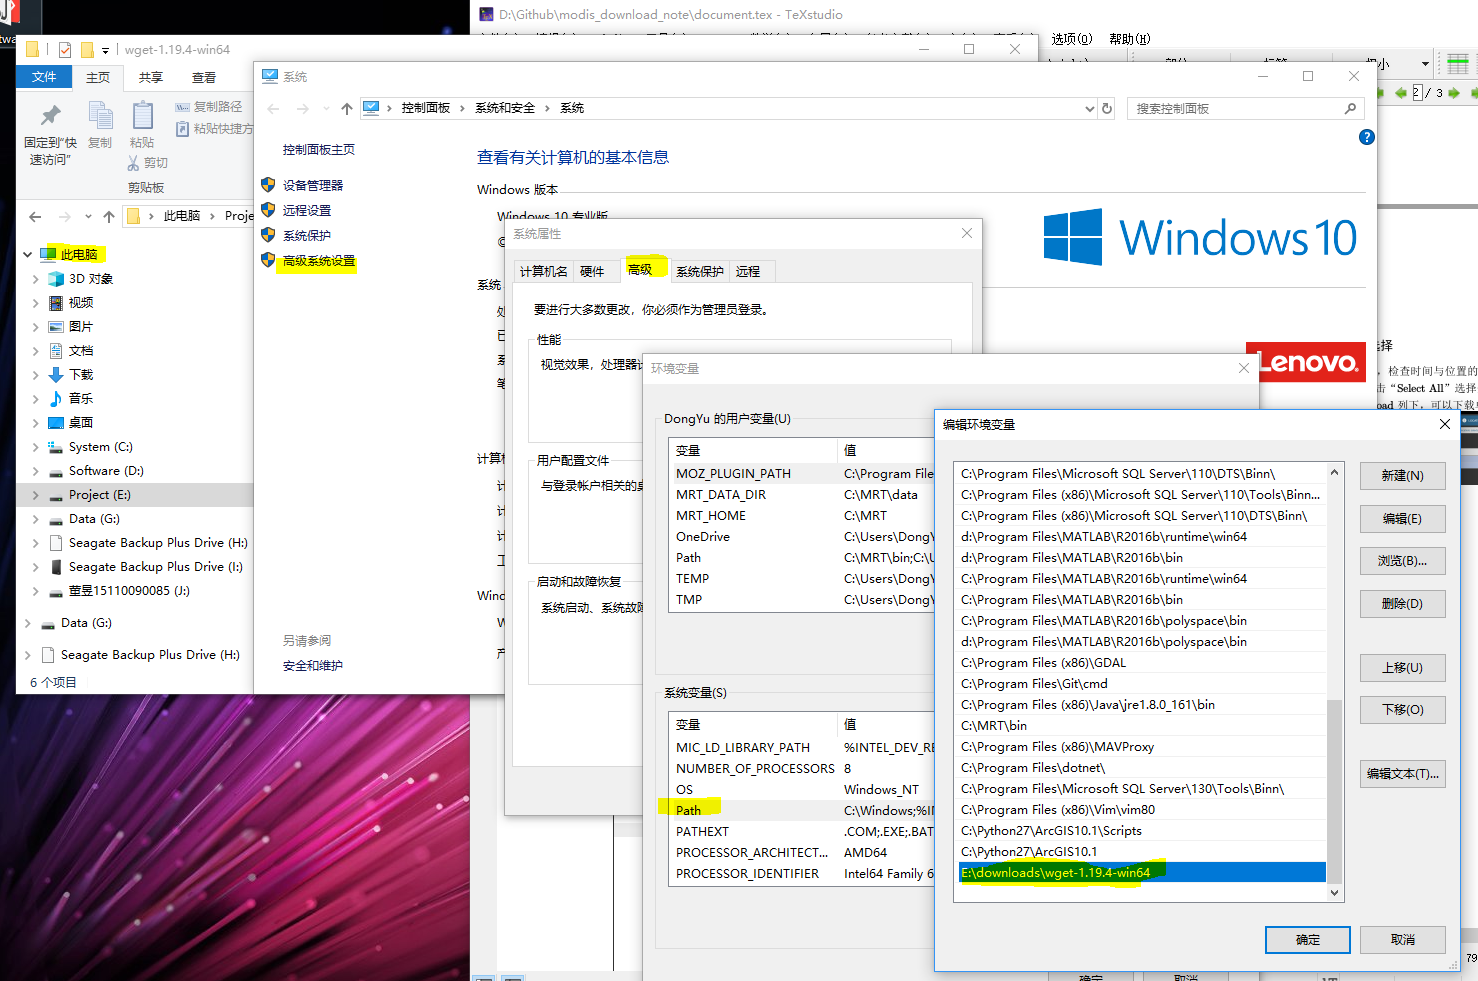
\includegraphics[width=\linewidth]{sec3_2.png}
	
	按下Ctrl+R按钮,打开"运行"对话框,输入cmd回车打开命令提示符。在命令提示符中输入wget --version回车,如果出现wget版本号,则表示配置成功。
	
	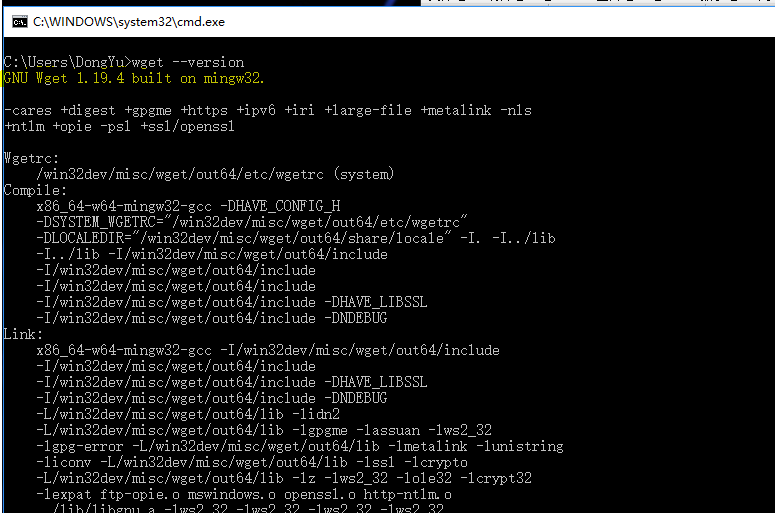
\includegraphics[width=\linewidth]{sec3_3.png}
	
	
	\section{数据下载}
	
	打开NASA发来的订单成功的邮件,找到如下图所示的命令。
	
	
	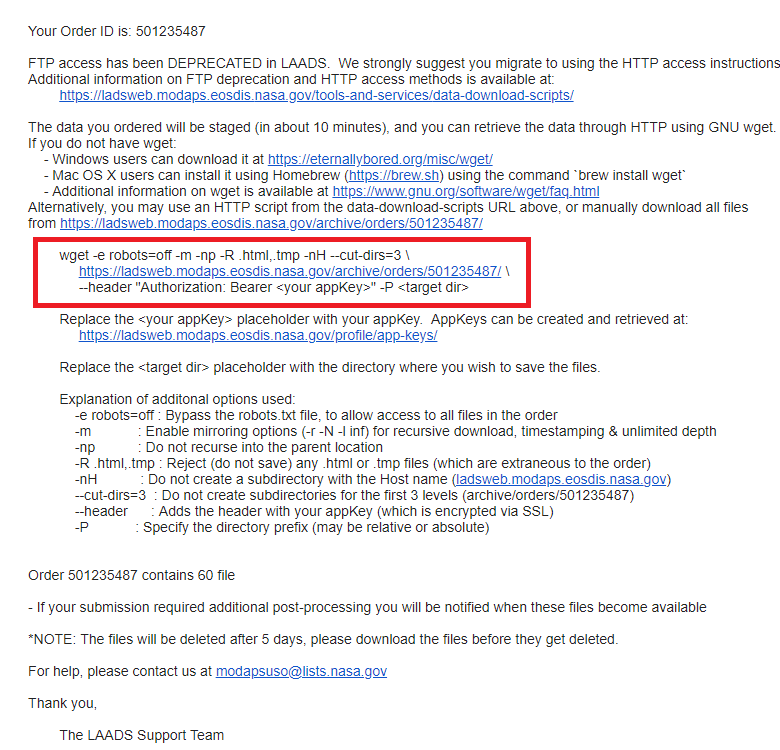
\includegraphics[width=\linewidth]{sec4_1.png}
	
	将这一条命令复制到文本文档中,进行如下操作:
	
	(1) 将所有的"$\backslash$"修改为"\^{}".
	
	(2) 将<your appKey>修改为第一步中的App Key.
	
	(3) 将<target dir>修改为数据的下载目录.
	
	如下图所示。
	
	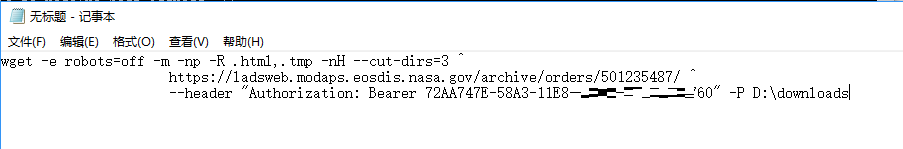
\includegraphics[width=\linewidth]{sec4_2.png}
	
	
	复制上面的命令,在命令提示符中单击鼠标右键粘贴,回车运行,出现下面的界面即为开始下载。
	
	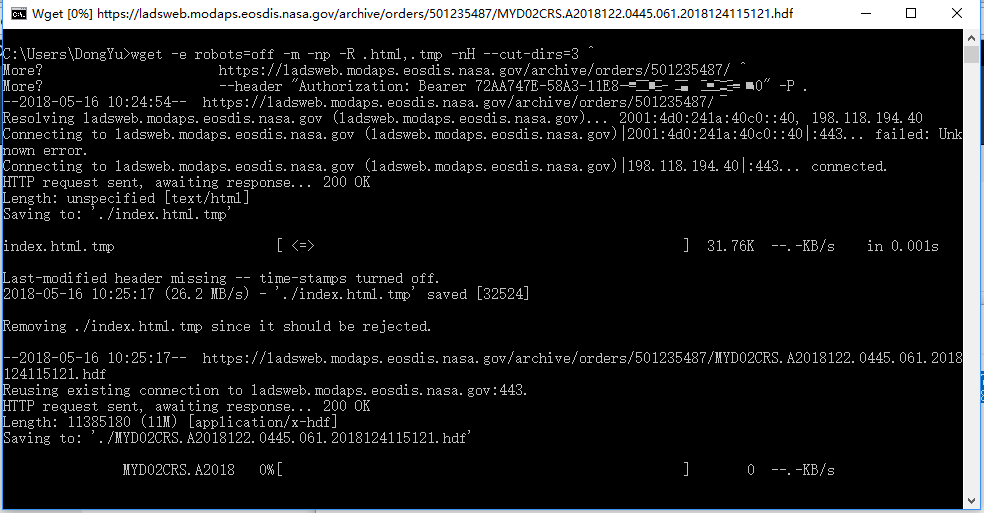
\includegraphics[width=\linewidth]{sec4_3.png}
	
\end{document}